\lstdefinestyle{yaml}{
     basicstyle=\color{red}\footnotesize,
     rulecolor=\color{black},
     string=[s]{'}{'},
     stringstyle=\color{red},
     comment=[l]{:},
     commentstyle=\color{black},
     morecomment=[l]{-}
 }
 \lstset{numbers=left}
 
\chapter{Cloud Infrastructure} \label{ch:AWSUsedServices}
As discussed in previous chapters, the development of SDV technology requires a cloud infrastructure to handle server-side operations. AWS is a leading player in the cloud world, and therefore an ideal alternative for the advancement of SDV, as well as an active partner in the implementation of technologies that contribute to the creation of a publicly available SDV for all. The following discussion introduces and analyzes, via AWS documentation the key tools for successful Proof of Concept (POC) implementation which will be explored in more detail later.

\section{AWS Used Services}
\begin{itemize}
    \item \textbf{AWS CLI} 
    
    The AWS Command Line Interface (CLI) is an essential tool for developing with AWS services. t allows interaction with AWS services from the command line of a local PC, enabling the creation of infrastructure and management of properties from the command line.
    
    \item \textbf{AWS Boto} 
    
    Boto is an AWS SDK made for Python. A software Development Kit (SDK), more generally, is a set of creation tools specifically for developing and running software in a single platform. It includes resources such as documentation, examples, and APIs to facilitate faster application development. Boto basically works as an interface for applications that need to interact with and take advantage of the services provided by AWS. The AWS SDK for JavaScript v3 is another example of an SDK for JavaScript that works basically in the same way.
    \begin{figure}[h]  % 'h' significa che la figura viene posizionata qui
        \centering
        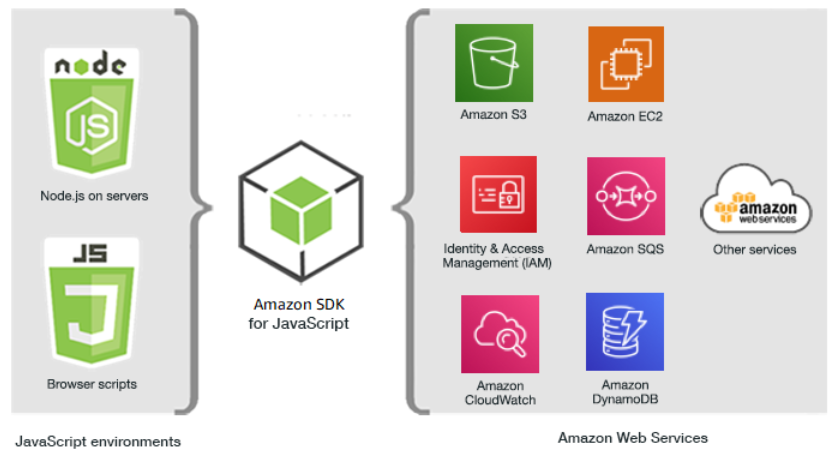
\includegraphics[width=0.8\textwidth]{images/AWSSDK.png}  % Sostituisci 'nome_immagine' con il nome del tuo file immagine e l'estensione
        \caption{The high level rappresentation of the AWS SDK for JavaScript v3 \cite{AWSSDK}}
        \label{fig:AWSSDK}
    \end{figure}
    
    \item \textbf{AWS CDK} 
    
    The AWS Cloud Development Kit (CDK) "is an open-source software development framework for defining cloud infrastructure in code and provisioning it through AWS CloudFormation" \cite{WhatIsTheAWSCDK}. This tool was used in the final phase of the POC design to automate the creation of the stack comprising all the services used.
    
    \item \textbf{AWS IoT Core} 
    
    AWS IoT Core provides the ability to connect IoT devices to AWS cloud services. AWS IoT Core enables the connection of IoT devices to AWS cloud services. It simplifies the integration of IoT devices with other AWS services. This is especially relevant in the automotive industry, where vehicle system ECUs can be viewed as multiple IoT devices. Communication between the device and AWS services can occur in several modes, with the MQTT protocol being the most important for this project. The device can be connected by developing applications that utilize the SDK libraries. Once the data is transmitted, it can be utilized for various purposes such as testing, validation, and analysis. The AWS IoT services, including the IoT Core service, allow for the creation of digital twins of physical IoT devices, known as Thing, and monitoring of traffic on selected MQTT channels. These elements will be explored in greater detail later in the PoC analysis.
    \begin{figure}[h]  % 'h' significa che la figura viene posizionata qui
        \centering
        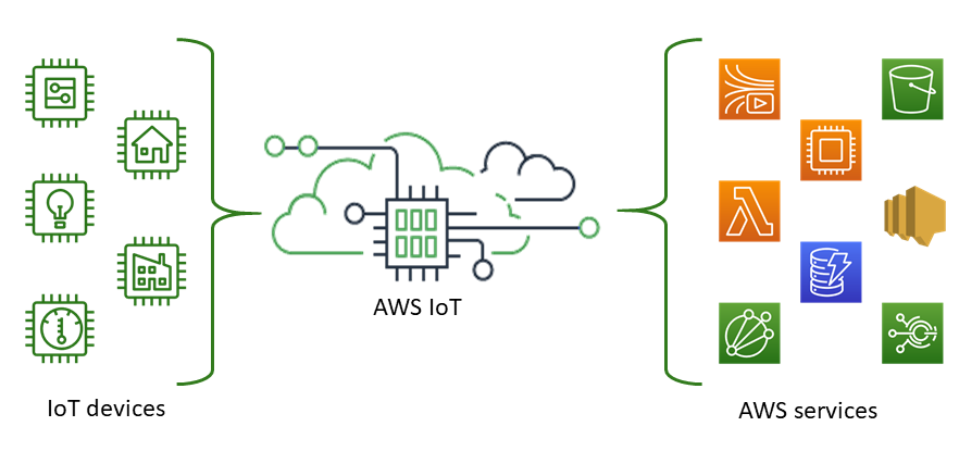
\includegraphics[width=0.8\textwidth]{images/AWSIoTCore.png}  % Sostituisci 'nome_immagine' con il nome del tuo file immagine e l'estensione
        \caption{AWS IoT Core connection system beetween IoT device and AWS service \cite{AWSIoTCore}}
        \label{fig:AWSIoTCore}
    \end{figure}

    \item \textbf{AWS IoT Greengrass}
    
    "AWS IoT Greengrass is an open source Internet of Things (IoT) edge runtime and cloud service that helps you build, deploy and manage IoT applications on devices" \cite{AWSIoTGreengrass}. It is designed to work with intermittent connections and can manage fleets of devices in the field, locally or remotely, using MQTT or other protocols. Once installed, this service can be accessed through the command line. It was utilized in the early stages of project development as an agent to handle updates on the vehicle simulator side. However, this solution will be replaced by a custom solution as explained later.
    
    \item \textbf{AWS IAM}
    
    "AWS Identity and Access Management (IAM) is a web service for securely controlling access to AWS services [...] such as access keys, and permissions that control which AWS resources users and applications can access" \cite{AWSIAM}. IAM is a service that provides a powerful access management mechanism. However, for the purpose of this thesis, only the relevant functionality to the project will be analyzed, specifically IAM's role management capabilities.An IAM role is an identity within AWS that can be assigned specific permissions via permission policies to determine what actions can and cannot be taken. Roles can be assumed by users, applications, or services that do not normally have access to the specific AWS resources. The IAM service also provides another important concept, that of policy, which is an AWS object that, when attached to an identity (including roles) or a resource, enables the creation of permissions and access control to other resources. For example, as explained below, a policy can be attached to the cloud representation of an IoT Core device to enable the connection of the physical dual IoT device or to grant Subscriber or Publisher permissions in a communication via MQTT protocol.
    \item \textbf{AWS Lambda}
    
    AWS Lambda is a computing service that provides the ability to run code without servers. It runs code on a high-performance computing infrastructure and handles administrative tasks related to computing resources autonomously, such as server and operating system management, capacity provisioning, automatic scaling, and logging. It is possible to run code for potentially any type of backend application or service \cite{AWSLambda}. Code can be written directly in Lambda console or imported from the local environment, and it supports several languages, including Python and JavaScript. The Lambda service can also manipulate data from other AWS services or manage tasks with services outside AWS as will be analyzed below.
    \item \textbf{AWS Codepipeline}
    
    AWS CodePipeline is a fully managed continuous delivery service that automates release pipelines for software updates. It enables fast and reliable updates to applications and infrastructure, facilitating the rapid release of new features, iterative development based on feedback, and bug detection through testing every code change. The software release process can be modeled and configured quickly via the stages execution. A stage is a logical unit that creates an isolated environment and allows for the execution of a limited number of concurrent software changes. Each stage contains actions that are executed on application artifacts, such as source code from Codecommit. For instance, as shown in the image \ref{fig:AWSCodepipeline}, it is feasible to establish a software development pipeline that incorporates a codecommit repository as its source stage. This way, a codecommit-related event triggers the pipeline execution which then proceeds to the software build stage. An execution is defined as a series of modifications released from a pipeline.   Each execution represents a set of modifications, such as a merged commit or a manual release of the last commit. Subsequently, the pipeline moves on to the test stage where the desired tests can be launched via Codebuild, and finally delivers the application for production. 
    \begin{figure}[h]  % 'h' significa che la figura viene posizionata qui
        \centering
        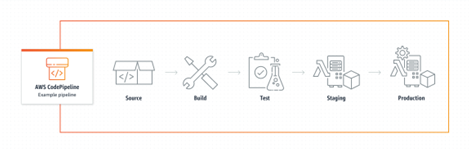
\includegraphics[width=0.8\textwidth]{images/AWSCodepipeline.png}  % Sostituisci 'nome_immagine' con il nome del tuo file immagine e l'estensione
        \caption{An example of a CodePipeline in which some stages are reported \cite{AWSCodepipeline}}
        \label{fig:AWSCodepipeline}
    \end{figure}
    \item \textbf{AWS Codebuild}
    
    AWS CodeBuild is a fully managed build service in the cloud that provides source code compilation, unit testing, and production of executable programs ready for distribution \cite{AWSCodebuild}. CodeBuild provides out-of-the-box configuration of compilation environments for popular programming languages, such as Python. It is also possible to create build platforms for programming languages for which there is no preconfiguration, but in this case it is necessary to leverage multiple AWS services. It is also possible to use codebuild to run tests on application code using for example the pytest tool that allows you to test python code.
    
    \item \textbf{AWS Codecommit}
    
    "AWS CodeCommit is a version control service that enables you to privately store and manage Git repositories in the AWS Cloud" \cite{AWSCodecommit}. This service becomes particularly interesting in the context of multiple services working together, including Lambda, Codepipeline, and Codebuild, because it allows the repository's Git and all its associated events (such as commit and push) to be used to trigger events that can automate various operations, such as triggering a pipeline in Codepipeline. As a result, CodePipelines typically use a CodeCommit repository as their inputo Source stage.
    
    \item \textbf{Amazon S3}
    
    "Amazon Simple Storage Service (Amazon S3) is an object storage service that offers industry-leading scalability, data availability, security, and performance" \cite{AWSamazonS3}. The data saved in the storage is physically placed in multiple locations to ensure the durability of the data even if there is tampering with an item due to the presence of these copies; optionally, it can also be chosen to store the data in a single location to reduce the cost of the service. Amazon S3 can be used for data collection, aggregation, and analysis in many contexts and scenarios, but in the scope of this project, this service is used to store data that is transferred from one stage of the Codepipeline to another. Amazon's Codepipeline service automatically implements this method of output use. However, data stored in S3 from one stage to another can be manipulated through integration with other AWS services, such as Lambda.
    \begin{figure}[h]  % 'h' significa che la figura viene posizionata qui
        \centering
        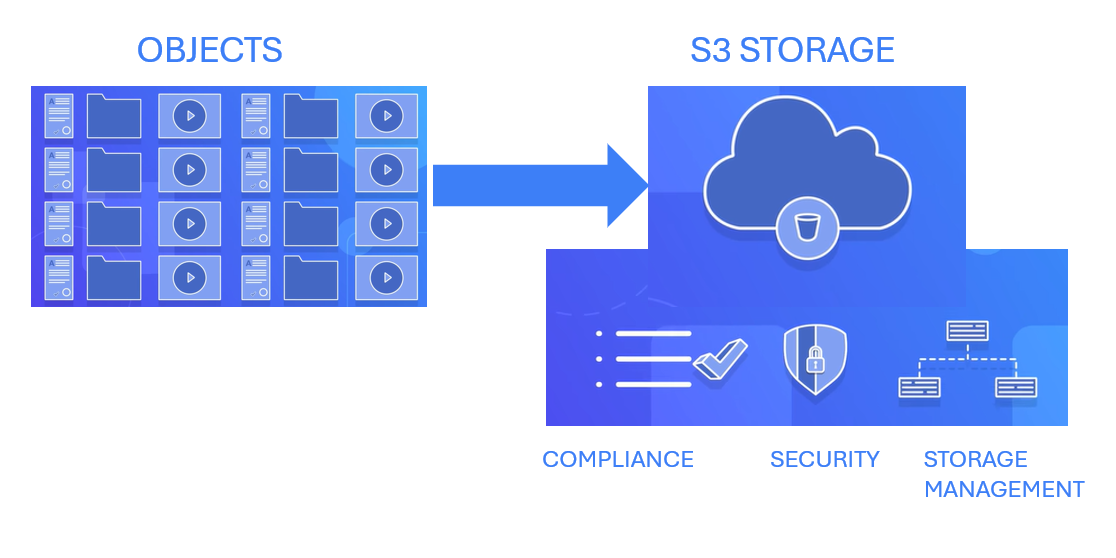
\includegraphics[width=0.8\textwidth]{images/AWSS3.png}  % Sostituisci 'nome_immagine' con il nome del tuo file immagine e l'estensione
        \caption{Amazon S3 high level storing rappresentation}
        \label{fig:AWSS3}
    \end{figure}
    
    \item \textbf{Amazon ECR}
    
    "Amazon Elastic Container Registry (Amazon ECR) is an AWS managed container image registry service that is secure, scalable, and reliable. Amazon ECR supports private repositories with resource-based permissions using AWS IAM. This is so that specified users or Amazon EC2 instances can access [...] container repositories and images" \cite{AmazonECR}. Basically, as shown in the figure \ref{fig:AWSECR}, once the software has been produced and packaged, for example through the use of the CodeBuild service, it can be uploaded to Amazon ECR. The ECR takes care of encrypting the image and controlling access to it, and then automatically manages the entire lifecycle of the image. Once the image is on ECR, it can be used either as an image for local download or through other AWS services. 
    \begin{figure}[h]  % 'h' significa che la figura viene posizionata qui
        \centering
        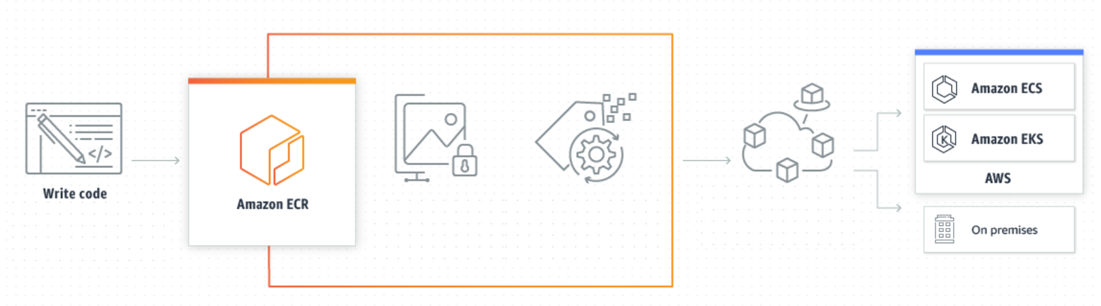
\includegraphics[width=0.8\textwidth]{images/AWSECR.png}  % Sostituisci 'nome_immagine' con il nome del tuo file immagine e l'estensione
        \caption{Example of how Amazon ECR works in production and for pulling images \cite{AWSECR}}
        \label{fig:AWSECR}
    \end{figure}
    
    \item \textbf{EC2}
    
    Amazon Elastic Compute Cloud (Amazon EC2) provides scalable, on-demand computing capacity in the Amazon Web Services (AWS) cloud. With Amazon EC2, users can create and use virtual machines in the cloud, instantiating resources as needed to perform compute operations. Amazon EC2 is a common choice for rapidly deploying applications because it provides an excellent computing resource at a low cost \cite{AWSEC2}, and it is possible to manage networks of different instances of EC2 virtual machines through Amazon Virtual Private Cloud (VPC) and set their relative security, either on a per-instance basis or on an overall network basis. Additionally, it is possible to increase the capacity (scale up) of the instance after creation to handle computationally heavy tasks, such as spikes in website traffic. Conversely, if utilization decreases, capacity can be reduced (scale down). EC2 instances can be launched with Amazon Machine Images (AMIs), which are preconfigured templates containing the necessary components to use the server, including the operating system and additional software. AWS provides pre-built AMIs, but it is also possible to create your own AMIs using containers. Furthermore, it is possible to connect to an EC2 instance through various communication systems, such as using SSH keys provided at the time of instance creation.
    
    \item \textbf{AWS System Manager}
    
    AWS Systems Manager is a service that provides visibility and control of the infrastructure on AWS.  It allows users to view operational data from multiple AWS services and manage the automation of operational tasks across different AWS resources \cite{AWSSM}. The AWS System Manager service is particularly relevant to the project due to its application management capability, namely the Parameter Store. Parameter Store is used to securely store configuration data and secrets, such as passwords, connection strings, and Amazon Machine Image (AMI) identifiers. Values are stored hierarchically by assigning hierarchical names to stored values using the "/" character, while maintaining the uniqueness of the name. For example, names such as Parameters/Parameter1, Parameters/Parameter2 can be used. In addition, it is possible to choose whether to store the data as plain text or encrypted data. Stored data can be retrieved directly from other services, for example, by interacting with Lambdas and SDK code functions.
    
    \item \textbf{Amazon Kinesis Data Streams}
    
    Amazon Kinesis Data Streams is used to collect and process large streams of data records in real time, and eventually route them through other AWS services to various data collection and analysis applications, such as Amazon S3 as it is shown in the image \ref{fig:AmazonKinesis}. "The delay between the time a record is put into the stream and the time it can be retrieved (put-to-get delay) is typically less than 1 second. In other words, a Kinesis Data Streams application can start consuming the data from the stream almost immediately after the data is added" \cite{AWSKinesis}. The Kinesis Data Stream service allows for the selection of specific data based on characteristics through an integrated query system. Additionally, this service can serve as input for lambda functions or to populate databases. 
    \begin{figure}[h]  % 'h' significa che la figura viene posizionata qui
        \centering
        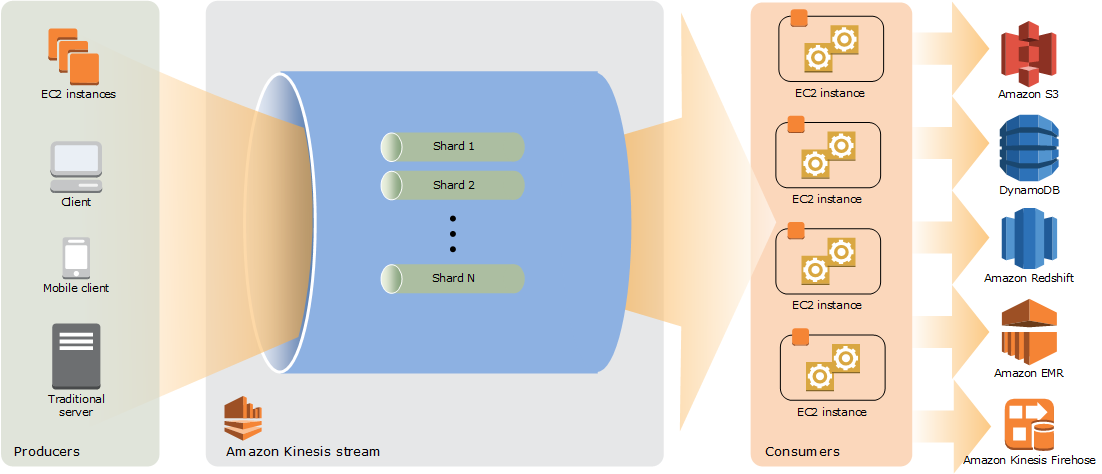
\includegraphics[width=0.8\textwidth]{images/AmazonKinesis.png}  % Sostituisci 'nome_immagine' con il nome del tuo file immagine e l'estensione
        \caption{Illustration of the high-level architecture of Kinesis Data Streams with some examples of services that use the output of the stream. \cite{AmazonKinesis}}
        \label{fig:AmazonKinesis}
    \end{figure}
    
    \item \textbf{Amazon Timestream}
    
    Amazon Timestream is a time-series database that allows you to store and easily analyze large amounts of data stored at regular intervals, ensuring that the time-series data is always encrypted, whether at rest or in transit. This service simplifies the complex process of managing the lifecycle of data by providing storage tiering with an in-memory store for current data and a magnetic store for historical data using Amazon S3 space. The transition of data between these two storage types is enabled through the use of user-configurable policies. The data lifecycle management mechanism makes Amazon Timestream ideal for handling telemetry data from IoT devices, for example. The service also provides a built-in interface for accessing data through a query engine \cite{AWSTimestream}. The Timestrem service also provides an interface for Grafana to view and analyze stored data, which will be explored later.
    
    \item \textbf{DinamoDB}
    
    Amazon DynamoDB is a full-featured NoSQL database service that provides high perfomances both speed and scalability. DynamoDB removes the administrative complexity of running and scaling your distributed database, so there's no need to manage provisioning, hardware setup and configuration, replication, software patching, or cluster sizing. DynamoDB also provides encryption at rest, eliminating the operational costs associated with protecting sensitive data. DynamoDB provides the ability to change the allocation of resources needed to store data in real time to use only the resources required. Additionally, DynamoDB offers on-demand backup functionality for long-term retention and archival purposes, as well as point-in-time recovery to safeguard against accidental write or delete operations. This feature enables users to restore a table to any point within the last 35 days \cite{AWSDynamoDB}. Note that this service was not utilized in the final version of the project, but was considered during development as an alternative for data storage and as a case study for understanding the data storage mechanisms used by AWS services.
    
    \item \textbf{Amazon Cloudwatch}
    
    Amazon CloudWatch is a system to monitor the Amazon Web Services (AWS) resources and the applications running on the infrastructure in real time. With the use of CloudWatch it is possible to collect and track metrics from other AWS services such as Lambda, which are numeric variables that can be measured and analyzed for resources applications \cite{AWSCloudwatch}. Practically this service represents the center for viewing and analyzing logs from the various AWS services in use.
\end{itemize}

All of the previously listed services have been useful, both as an active part in the project's realization and as potential options for the project's implementation, which will be analyzed below. 

After reviewing the various services theoretically, it is now possible to understand a high-level look at how the various services interact with each other.
The interaction system is intricate and consists of two main circuits. The image \ref{fig:AWSDataServices} shows the management of data from the TCU edge device in the first part. The data is sent to the cloud via the IoT Core thing, inserted into a Kinesis channel, and then sent to a Timestream database in relevant tables.
\begin{figure}[h]  % 'h' significa che la figura viene posizionata qui
    \centering
    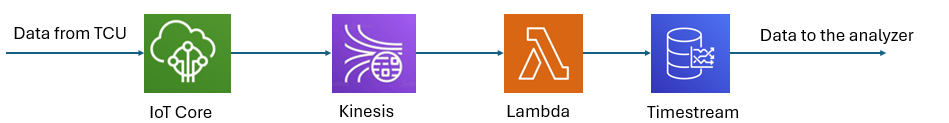
\includegraphics[width=1\textwidth]{images/AWS_data_services.png}  % Sostituisci 'nome_immagine' con il nome del tuo file immagine e l'estensione
    \caption{The high level rappresentation of the ASW services for the data managing}
    \label{fig:AWSDataServices}
\end{figure}

\begin{figure}[h]  % 'h' significa che la figura viene posizionata qui
    \centering
    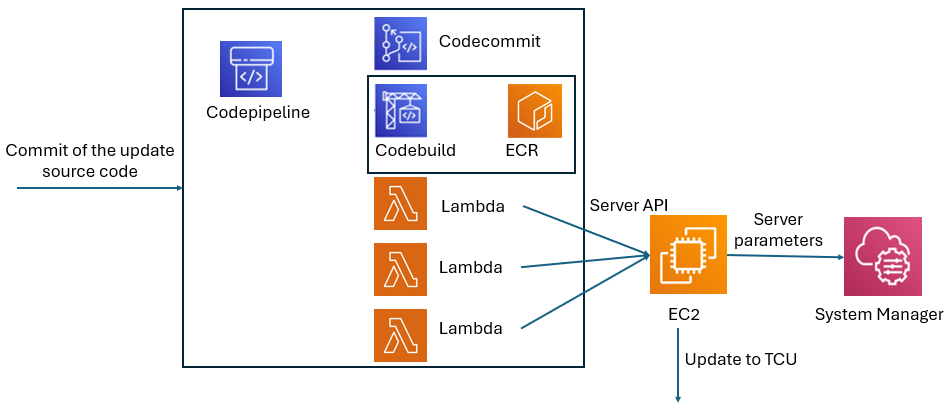
\includegraphics[width=1\textwidth]{images/AWS_update_services.png}  % Sostituisci 'nome_immagine' con il nome del tuo file immagine e l'estensione
    \caption{The high level rappresentation of the ASW services for the update managing}
    \label{fig:AWSUpdateServices}
\end{figure}
During the second part of the service interaction shown in the image \ref{fig:AWSUpdateServices}, the system consists of a Codepipeline that can be triggered by a Codecommit event acting as a source. The pipeline includes a build phase via Codebuild, which can utilize images from ECR registries, followed by three phases consisting of Lambda functions. The pipeline interacts with a server located on an EC2 instance, which stores its key information in the parameter Stor of the System Manager service.

The components of the cloud structure may appear separate, indeed there is no actual interaction between data management services and update management services. However, the TCU device serves as the point of connection. It continuously sends data to the cloud, which can be analyzed, and receives updates. This process can continue indefinitely.

The following section provides a detailed analysis of the PoC structure, covering the edge device, cloud infrastructure, their connection, and data analysis system.